

\section{Results}

\subsection{Position dependence}

Figure \ref{fig:pos_dependence_aes} shows the results of the position-dependent AES2 measurements. Figure \ref{fig:pos_dependence_aes}A shows the AES2 absorption spectra for a few positions along the free jet, along with fits. Figure \ref{fig:pos_dependence_aes} B and C show the potassium number density obtained from the $\alpha$ fit for different positions along the torch axis, and 0.8 and 0.6 equivalence ratio. The potassium measurement at the barrel exit throughout the position sweep is also shown. The CFD data is sampled along a line on the torch axis, either directly on the torch axis or offset perpendicular to simulate misalignment in the AES2 beam. 

% As discussed above, inaccuracies in the AES calibration can cause offsets to appear in $\alpha$ which are visible in the raw data presented in \ref{fig:pos_dependence_aes}A. Our procedure for fit preparation corrects for these offsets while preserving the peak absorption profile. This procedure, other fit preparation, and details of the fit are discussed in the SI. 


\begin{figure}[h]
    \centering
    
\includegraphics[width=0.8\linewidth]{\repodir/final/figures/output/Fig3_Position_AES.png} 
    \caption{AES Measurements: A) AES absorption spectra and fits for a few positions along the free jet. B) Position dependence of atomic potassium $n_{K,cl}$ as measured by AES and predicted by CFD for 1 \% seed and an nominal equivalence ratio of 0.8. The CFD data is sampled along a line on the torch axis, either directly on the torch axis or offset perpendicular to simulate misalignment in the AES beam. C) The same as B, but for a nominal equivalence ratio of 0.6. }
    \label{fig:pos_dependence_aes}
\end{figure}

Figure \ref{fig:pos_dependence_mws} examines the position dependence of the MWS signal at a fixed 1 \% potassium mass fraction.  These measurements are now used to motivate the nominal stage position of 180 mm downstream of the jet which is used for the fixed position Kwt dependence measurements presented in the next section. Figure \Ref{fig:pos_dependence_mws}A and B show the $\Delta AS$ signal at a position of 105 mm and 180 mm downstream of the barrel exit, respectively. In Figure\ref{fig:pos_dependence_mws}A $\Delta AS$ time profiles for each Run are shown. We observe that near the exit of the torch (including the 105 mm position shown) there is a significant fluctuation in the MWS signal in the absence of a laser pulse. These fluctuations can be observed in the $\Delta AS$ signal, where the underlying transmission magnitude is fluctuating and causing the $\Delta AS$ signal to above and below the zero line. As mentioned previously, the $\Delta AS$ signal is calculated with respect to a time window of 1 $\mu s$ before the laser pulse, and therefore deviations in transmission magnitude prior to the laser pulse can cause the $\Delta AS$ signal to fluctuate below zero.


\begin{figure}[h]
    
\includegraphics[width=0.8\linewidth]{\repodir/final/figures/output/Fig4_Position_MWS.png} 
    \centering
    \caption{Position dependence of the MWS signal. The data are taken for full laser power and 1\% nominal K mass fraction. All error bars are standard deviation across Runs.  A) AS profiles taken at 105 mm downstream of the barrel exit The hue represents different runs of the test case, with each line being an average of all oscilloscope acquisitions.  B) The AS signal further downstream at the nominal position of 180 mm. The shaded region represents the standard deviation across runs C)  The maximum of the $\Delta AS_{max}$ signal, calculated as described in the text.  D) The SFR, calculated as described in the text.  For C, and D the error bars represent the standard deviation across runs. Vertical dashed lines represent the positions shown in A and B. Note that on 2023-05-12, position dependent measurements were performed on a different but semi-overlapping set of positions (including the nominal position), leading to the datapoints with zero error bars. } 
    \label{fig:pos_dependence_mws}
\end{figure}

For the present discussion, the important point is that these fluctuations are significant compared to the signal induced by the laser pulse, and they therefore preclude accurate measurement of the time decay of the AS signal after the laser pulse. The source of these fluctuations is not investigated in detail in the present work, but presumably the temperature at the exit of the torch is sufficiently high for thermally induced conductivity and we are observing fluctuations in this conductivity from turbulence or other variations such as inconsistencies in the emulsion composition.

In Figure \ref{fig:pos_dependence_mws}B the $\Delta AS$ signal is shown at 180 mm downstream of the barrel exit. The background fluctuations in the $\Delta AS$ signal are reduced compared to the 105 mm position, but a $\Delta AS$ response from the laser is still observed. In Figure \ref{fig:pos_dependence_mws}C we show the maximum of the $\Delta AS$ signal as a function of stage position, $\Delta AS_{max}$. $\Delta AS_{max}$ is calculated as the average of the $\Delta AS$ signal in a time window of 100 ns after the laser pulse. This method is chosen as there is some electromagnetic interference from the excimer laser within a few hundred nanoseconds of the laser pulse, and this time window averages approximately over a cycle of this interference while remaining small enough to capture the peak maximum (see Figure \ref*{fig:SI_MWS_nothing_T0}). $\Delta AS_{max}$ signal is interpreted as a measure of the signal strength and is observed to increase with stage position, and then decrease.

To determine the nominal location for measurement of the potassium dependence, we define a signal to fluctuation ratio (SFR): 

\begin{equation}
    \label{eq:sfr}
    SFR = \frac{\Delta AS_{max}}{U_{std,PP}}
\end{equation}

Where $U_{std,PP}$ is the standard deviation of the MWS magnitude in the time window of -50 to -1 $\mu s$ before the laser pulse, calculated before averaging over repeat acquisitions.  In figure \ref{fig:pos_dependence_mws}D we examine the SFR as a function of stage position to find the optimal position for the MWS diagnostic. We observe that similar to $\Delta AS_{max}$, $U_{std,PP}$ increases downstream of the torch, and decreases (TODO SI). However, $PP_{std}$ decreases more rapidly than $AS_{max}$, so the signal to fluctuation ratio increases to a maximum at approximately 180 mm downstream from the torch. 

The maximum of the SFR at 180 mm downstream of the barrel exit motivates the choice of this position for the Kwt dependence measurements presented in the next section. Measurements are taken at 180 mm downstream of the barrel in order to maximize the signal to fluctuation ratio and accurately measure the profile of the AS decay after the laser pulse. We therefore refer to 180 mm downstream from the jet as the \textbf{SFR-maximized position}. We note that the AS decay rate does not appear to depend sensitively on the position (see Figure TODO in the SI), which is discussed further later. 

Power dependence measurements are presented in Figure \ref{fig:SI_power_dependence}. We observe that $\Delta AS_{max}$ increases with laser power according to a power law $\Delta AS_{max} \propto P^{k}$, with a power law coefficient of $k = 2.05 \pm 0.04$. We further observe that the fitted exponential time constant of the AS decay does not depend sensitively on the laser power and the fitting becomes more reliable at high laser power. We therefore take measurements at full laser power (7 mJ) to maximize the $\Delta AS$ signal.


\clearpage

\subsection{Potassium dependence}

Figure \ref{fig:kwt_ionization} shows results with the mobile diagnostics positioned at 180 mm and full laser power, while varying the nominal potassium mass fraction. Figure \ref{fig:kwt_ionization}A shows the potassium number density, $n_K$, as measured by both AES diagnostics, compared to species densities predicted by CFD. The barrel measurement of the $n_K$ is observed to increase with the nominal potassium mass fraction, as expected. However, $n_K$ at the SFR-maximized position has a slight decrease as a function of increasing nominal mass fraction. The CFD predictions for K, KOH, and all K species are also shown.  The CFD K density at the SFR-maximized position is similar to the experimental results, and the K species sum at the SFR-maximized position is consistent with the AES2 measurements at the barrel. Additionally, nearly all K species are predicted to predicted to be in the form of KOH at the SFR-maximized position. Together, these results suggest that the temperature of the jet has reduced sufficiently that the potassium is primarily in the form of KOH at the SFR-maximized position.

Figure  \ref{fig:kwt_ionization}B shows $\Delta AS_{max}$ as well the on-peak PD signal as a function of nominal potassium mass fraction. The photodiode signal is from the on-peak (K filtered) photodiode and is the difference between the maximum of the signal in time and the signal 1 $\mu s$ before the laser pulse. Both signals are observed to increase with the nominal potassium mass fraction. 

\begin{figure}[h]
    \centering
    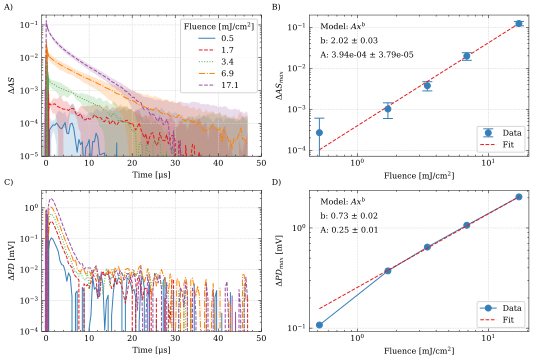
\includegraphics[width=0.8\linewidth]{\repodir/final/figures/output/Fig5_Kwt_Ionization.png} 
    \caption{Kwt dependence of Ionization related parameters. Measurements and predictions are for the free jet at the nominal position of 180 mm or exit of the HVOF barrel. measurements are for full laser power as a function of nominal potassium weight percent at 0.8 equivalence ratio. A) species number density results and CFD predictions. MWS $\Delta AS_{max}$ and photodiode signal. The photodiode signal is from the on-peak (K filtered) photodiode and is the difference between the maximum of the signal in time and the average of the signal 1 to 2 us before the laser pulse.  }
    \label{fig:kwt_ionization}
\end{figure}


Figure \ref{fig:kwt_recombination} shows analysis of the $\Delta AS$ decay measurements as a function of nominal potassium mass fraction.  Figure \ref{fig:kwt_recombination}A shows the $\Delta AS$ time profile for a range of K mass fraction. Immediately after the laser pulse, there is a region of of changing slope in the logarithm of the $\Delta AS (t)$ profile. After a few microseconds, the profile becomes an exponential decay. Finally, after approximately 20 $\mu s$ the AS fluctuations cause the signal to dip below zero and the measurement is not meaningful. Assuming, where the signal is above the level of AS fluctuations, that $\Delta AS (t) \propto \Delta n_e (t)$, where $\Delta n_e (t)$ is the time dependent change in the free electron density from the steady state concentration, we derive in the SI a differential equation for the decay of $\Delta n_e (t)$. In the regime where $\Delta n_e (t)$ is small, the equation has an exponential form.  

\begin{equation}
    \label{eq:fit_eq}
    \frac{d\Delta n_e (t)}{dt} = - k_{r, m, eff} \Delta n_e (t) 
\end{equation}

The time constant of the exponential decay for capture with species X, $\tau$, is given by

\begin{equation}
    \label{eq:tau_krm}
    k_{r, m, X} = \frac{1}{\tau} = k_{r, b, X}n_{X,0}
\end{equation}

Where, $\tau$ is the exponential time constant and $n_{X,0}$ is the equilibrium species concentration of X, and $k_{r, b, X}$ is the bimolecular recombination rate coefficient for capture by X. The fitted time constants are shown in Figure \ref{fig:kwt_recombination}B 


\begin{figure}[h]
    
\includegraphics[width=0.8\linewidth]{\repodir/final/figures/output/Fig6_Kwt_Recombination.png} 
    \centering
    \caption{Kwt dependence of the MWS decay. A) A representative MWS $\Delta AS$ time profile and exponential fit. The time profile is from 2023-05-12 Run 1. B) exponential time constants associated with equation \ref{eq:tau_krm}. The time constant is measured experimentally through and exponential fit of the AS signal. The CFD predictions are based on the literature rate constants and CFD species number densities at the SFR-maximized position as discussed in the text. C) The effective bimolecular recombination rate coefficient, $k_{r,eff}$, calculated from the measured decay and CFD-predicted oxygen concentration along with literature values for $k_{r,b}$ of the oxygen reaction calculated from Table \ref{tab:reactions} and CFD collisional partner species densities as described in the text. The average of the effective experimental bimolecular rate constant is $k_{r,eff} =  2.69 \times 10^{-13} cm^3/s$.}
    \label{fig:kwt_recombination}
\end{figure}


We have also tried fitting the decay through iterative least squares fitting of the entire decay profile with a normalized solution to the differential equation. The results are consistent with the exponential fit, but allow for determination of the initially created electron population. Further work is needed to determine the accuracy of this method but the results are presented in the SI (Figure \ref*{fig:SI_Kwt_Recombination_fitmethod_compare}) .

We calculate expected exponential time constants for recombination with various species in \ref{fig:kwt_recombination}B to compare to the experimental exponential time constant. The expected exponential time constants are calculated through equation \ref{eq:tau_krm} with $n_{X,0}$ given by the CFD results at the SFR-maximized position. For $k_{r,b,X}$, we have searched for data on reaction kinetics that are compatible with the observed first-order (exponential) recombination of electrons (eq. \ref{eq:fit_eq}) which are summarized in Table \ref{tab:reactions}. For K+ and $H_2O$, and $k_{r,b,X}$ is given directly in the literature in units of $cm^3/s$. For $O_2$ and OH, the rates are are termolecular and further depend on a collisional partner, M, and are of the form [X] +[e-] + M \rightarrow [X-] + M. in this case $k_{r,b} = k_{r,tm} [M]$, where $k_{r,tm}$ is the termolecular recombination rate given in units of $cm^6/s$ and [M] is the number density of the collision partner.  The species density [X] is taken from the CFD results at the SFR-maximized position and we use the number density of all species in the flame as the density for [M]. 


\begin{table}[h]
\centering
\caption{Collected Reaction Kinetics for Electron Recombination.}
\label{tab:reactions}
\begin{tabular}{|c|c|c|c|}
\hline
Name & Reaction & Rate Coefficient & Reference \\
\hline
K$^+$ & K$^+$ + e$^-$ + M $\rightarrow$ K + M & $4 \times 10^{-24}$ T$^{-1}$ cm$^3$/s & Jensen 1978 \\
\hline
O2\_A & O$_2$ + e$^-$ + M $\rightarrow$ O$_2^-$ + M & $5 \times 10^{-31} cm^6/s$ & Axford 1997 \\
\hline
O2\_B & ""                                          & $6 \times 10^{-34} cm^6/s$ &  Goodings 1979 \\
\hline
O2\_C & ""                                          & Weighted sum  &  Axford 1997 \\
\hline
OH & OH + e$^-$ + M $\rightarrow$ OH$^-$ + M & $3 \times 10^{-31}$ cm$^6$/s & Axford 1997 \\
\hline
H$_2$O & H$_2$O + e$^-$ $\rightarrow$ H$_2$O$^-$ & $1.6 \times 10^{-6}$ exp(36060/T) cm$^3$/s & Axford 1997 \\
\hline
\end{tabular}
\end{table}

For recombination with molecular oxygen, there is significant uncertainty in the rate constant and we consider a few possibilities indicated in the legend of \ref{fig:kwt_recombination}C. Axford 1997 discussed this uncertainty and presented a range of rate constants ultimately deciding on a value of $5e-31 cm^6/s$ for their H2 + O2 + N2 flame, which we consider as '$O2_A$'. In the same discussion they specify the dominant collisional partners of the various literature values of the rate constant, and for '$O2_C$' we preform a sum of species dependent $k_{r,tm}$ with the CFD number densities for each collisional partner to determine an overall $k_{r,b}$. The constants presented by Axford 1997 include low temperature measurements, but mention that the experimental results suggest that $k_{r,b}$ is expected to decrease at flame temperatures. Goodings 1979 indeed found a much lower rate constant for similar flames and speculated a large negative temperature coefficient for the oxygen capture reaction. We consider this as '$O2_B$' and use the number density of all species as the collisional partner density.   

Our experimental results for the exponential time constant fall within this large deviation. As discussed later, there are additional lines of evidence to suggest that oxygen molecules are the dominant recombination partner under the conditions of Figure \ref{fig:kwt_recombination}C. Assuming that oxygen is the dominant recombination partner, we can calculate and effective bimolecular recombination coeffect, $k_{r,b,eff}$, from the measured decay and CFD-predicted oxygen concentration. This is shown in Figure \ref{fig:kwt_recombination}C. The effective bimolecular rate constant is calculated as $k_{r,b,eff} = 1/\tau n_{O2,0}$, where $\tau$ is the measured exponential time constant and $n_{O2,0}$ is the CFD-predicted oxygen concentration at the SFR-maximized position. The average of the effective bimolecular rate constant is $k_{r,b,eff} =  2.69 \times 10^{-13} cm^3/s$, and this value is used in the viability analysis in the next section. We note that this value relies on the assumption that oxygen is the dominant recombination partner. $k_{r,b,eff}$ is observed to slightly increase ($\tau$ is slightly decreasing) with increasing potassium mass fraction, which would not be expected under this assumption. However, this change is small compared to the the difference in predicted exponential time constants for the various recombination partners.

In summary there is a large uncertainty in the $k_{r,b}$ for the oxygen capture reaction but our results fall within this large deviation. All other reactions predict decays much longer than the observed experimental decay. We note that the previously mentioned sources have much better agreement on the OH, H2O, and K capture reactions than the O2 capture reactions. 





